\documentclass[conference]{IEEEtran}
% \IEEEoverridecommandlockouts   % uncomment only if \thanks is needed
\usepackage{cite}
\usepackage{amsmath,amssymb,amsfonts}
\usepackage{algorithmic}
\usepackage{graphicx}
\usepackage{textcomp}
\usepackage{xcolor}
\usepackage{url}
\interdisplaylinepenalty=2500

\begin{document}

\title{Rate-Distortion Loss Attribution for AV1\\ Intra Partition Decisions}

\author{\IEEEauthorblockN{Pablo Rosa}
\IEEEauthorblockA{\textit{Video Technology Research Group (ViTech)} \\
\textit{Federal University of Pelotas} \\
Pelotas, Brazil \\
pablo.rosa@inf.ufpel.edu.br}
\and
\IEEEauthorblockN{Daniel Palomino}
\IEEEauthorblockA{\textit{Video Technology Research Group (ViTech)} \\
\textit{Federal University of Pelotas} \\
Pelotas, Brazil \\
dpalomino@inf.ufpel.edu.br}
\and
\IEEEauthorblockN{Marcelo Porto}
\IEEEauthorblockA{\textit{Video Technology Research Group (ViTech)} \\
\textit{Federal University of Pelotas} \\
Pelotas, Brazil \\
porto@inf.ufpel.edu.br}
\and
\IEEEauthorblockN{Luciano Agostini}
\IEEEauthorblockA{\textit{Video Technology Research Group (ViTech)} \\
\textit{Federal University of Pelotas} \\
Pelotas, Brazil \\
agostini@inf.ufpel.edu.br}
}

\maketitle

\begin{abstract}
The AOMedia Video 1 (AV1) codec decides how to split each intra-frame super block
through a recursive search that evaluates ten partition shapes per node, and
learned pruners are the dominant strategy to shorten that search. Every such
pruner couples the quality of the source that scores a node with the
aggressiveness of the policy acting on that score, so the reported time savings do
not identify which information carries the decision. This paper presents an
offline attribution protocol for AV1 intra partitioning that reads the
rate-distortion loss of competing representations at matched search-cost
reduction. The protocol fixes one pruning policy, sweeps its confidence threshold,
and charges each forced decision the overhead recorded by an exhaustive reference
search, so that representations are compared at the same amount of work skipped.
Experimental results over 3.81 million held-out decision nodes show that
twenty-four compact descriptors reduce the loss
of isolated block variance by 7.0 times, that eight causal partitioning columns
reduce it by a further 1.60 times, and that four quantization and position columns
add nothing. A ConvNeXt with 28.1 million parameters reading raw pixels stays 4.1
times behind the compact descriptors, which hold 2481 times fewer parameters, and
doubling its fusion width makes it worse. The protocol is ordinal and does not
convert into Bjontegaard delta bitrate. To the best of the authors' knowledge,
this is the first work to attribute rate-distortion loss to information access in
AV1 partitioning under matched cost.
\end{abstract}

\begin{IEEEkeywords}
Video coding, AV1, intra-frame partitioning, feature representation, model
capacity, machine learning.
\end{IEEEkeywords}

\section{Introduction}

Video coding removes the spatial and statistical redundancy of a raw sequence so
that it can be stored and transmitted at a small fraction of its original rate.
Every coding choice trades bitrate against reconstruction fidelity, and encoders
resolve that trade-off by rate-distortion optimization, selecting at each decision
the candidate of lowest Lagrangian cost \cite{sullivan1998}. Coding efficiency is
the fidelity obtained at a given rate, and it degrades whenever a decision is
taken without evaluating the candidate that the full search would have selected.
That degradation, and not encoding time, is the quantity this work measures.

Two families of codecs pursue that efficiency. The standardization path produced
High Efficiency Video Coding \cite{hevc} and Versatile Video Coding \cite{vvc},
both developed jointly by ISO/IEC MPEG and ITU-T VCEG, while the Alliance for Open
Media released the AOMedia Video 1 (AV1) in 2018 as an open and royalty-free codec
\cite{av1site}, drawing on VP9, Thor, and Daala.

AV1 follows the hybrid block-based coding flow, combining intra-frame and
inter-frame prediction, transforms, quantization, in-loop filters, and entropy
coding, and it introduced new tools at every one of those stages
\cite{han2021,chen2018}. Among them, the partition structure was extended to ten
shapes per node, against the four of VP9. That coding efficiency is paid for in
computational effort, and comparative studies report AV1 encoding times far above
those of its competitors \cite{grois2016,layek2017}, with the gap widening at the
highest quality configuration.

Inside intra-frame coding, the recursive partition search is the single most
expensive stage at that configuration. The search visits a quad-tree of square
nodes, evaluates up to ten shapes at each one, and descends into every node it
does not resolve, so the cost grows with the number of nodes rather than with the
difficulty of the content.

Several works attack this cost with learned decisions. In AV1, tool selection
guided by user priority and by coding efficiency was proposed in
\cite{xu2020,xu2021}, a fast intra mode decision based on the accuracy of a
rate-distortion model in \cite{jeong2019}, and decision trees for inter prediction
in \cite{kim2019}. The same problem in Versatile Video Coding was addressed with
light gradient boosting \cite{saldanha2022}, random forests \cite{he2021}, and
variance and gradient heuristics \cite{chen2019}, while dedicated hardware
architectures targeted the AV1 intra prediction modes \cite{correa2020,netto2022}.
These works can be classified as coding-efficiency oriented
\cite{jeong2019,xu2021,saldanha2022,he2021,chen2019}, hardware oriented
\cite{correa2020,netto2022}, or aimed at a different coding stage
\cite{xu2020,kim2019}. All of them report time savings under a policy of their
own choosing, and none of these works separates the quality of the scoring source
from the aggressiveness of the policy, nor measures which information is decisive
for the partition choice.

This paper presents an offline attribution protocol for AV1 intra partitioning.
The main strategy of this work is to hold the pruning policy and the amount of
skipped search work fixed, and to vary only what a representation is allowed to
see, so that the
resulting difference in rate-distortion loss is attributable to information access
alone. Under this protocol, compact descriptors outperform a high-capacity
convolutional model reading raw pixels, and the causal partitioning neighborhood
carries decision information that luminance does not provide.

\section{Intra Partition Search in AV1}

AV1 partitions each frame into super blocks of 128$\times$128 samples, which the
encoder may alternatively set to 64$\times$64 \cite{han2021}. Each super block is
recursively divided by a search over a quad-tree of square nodes that may descend
to 4$\times$4 samples. At every node the encoder may evaluate ten partition
shapes, organized in four groups: the undivided block \texttt{PARTITION\_NONE},
the quaternary \texttt{PARTITION\_SPLIT}, the two rectangular shapes, and the six
extended shapes, which comprise four AB shapes and two four-way shapes.

The evaluation order inside a node is fixed: \texttt{PARTITION\_NONE} first, then
\texttt{PARTITION\_SPLIT}, whose opening triggers the recursion into the four
children, then the rectangular shapes, and the extended shapes last.

This order defines when each kind of information becomes available, the property
this work exploits. Before the search of a node begins, the encoder already holds
the source luminance of the block, the frame quantization index, the position of
the node, and the partition decisions of the causal neighbors above and to the
left, but it does not yet hold any rate-distortion cost for the current
node. Fig.~\ref{fig_timeline} summarizes this timeline.

The action studied in this paper is the earliest one available: committing the
node to the undivided shape before any rate-distortion evaluation is paid, and
therefore skipping every remaining candidate of the node and the whole subtree
below it. This single action has two measurable consequences, the search work that
is no longer performed and the rate-distortion cost that is lost whenever the
discarded subtree was the optimal choice.

This work is focused on that commitment at the pre-search insertion point of the
intra-frame partition tree. Inter-frame prediction, transform type selection,
quantization, in-loop filters, and entropy coding are not included in the loop
attacked here, and therefore they are not focused on this work. The decision at
the 128$\times$128 root is also outside this scope: the protocol attaches at the
four 64$\times$64 quadrants of each super block and models the 64, 32, and 16
sample levels. Blocks of 8$\times$8 samples were never split in this dataset, no
divided label appearing among 16.91 million of them, so 4$\times$4 nodes do not
occur and 8$\times$8 is the effective leaf; they are excluded from modeling while
kept in the cost accounting.

\begin{figure}[!t]
\centering
% Grayscale variant. The color one is figura1_linha_do_tempo.pdf, same geometry;
% both from src/scripts/benchmark/plot_information_timeline_icassp_fig1.py.
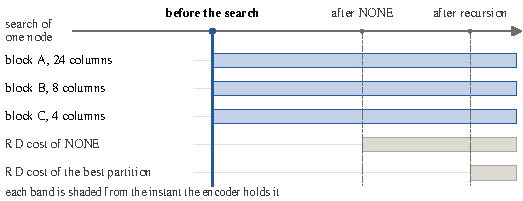
\includegraphics[width=\columnwidth]{fig1_information_timeline}
\caption{Information availability inside the search of one node: search time on
the horizontal axis, information item on the vertical.}
\label{fig_timeline}
\end{figure}

\section{Proposed Attribution Protocol}

The proposed protocol compares representations by what they are allowed to see,
under one fixed pruning policy and at a matched amount of skipped search work.

\subsection{Representations Declared by Information Access}

The representations are declared by information access rather than by
architecture. The first is the isolated variance of the block, the classical
descriptor of partition heuristics. The second, denoted A, is a twenty-four column
vector of compact luminance descriptors: second-order and gradient statistics of
the block and of its quadrants, edge measures, and the contrast against its parent
and sibling blocks. Three of those columns do not derive from luminance, namely
the normalized quantization index and the two coordinates of the node inside the
64-sample unit.

Block B adds eight columns of causal partitioning neighborhood: availability of
the above and left neighbors, their already decided widths and heights in
logarithmic scale, the relative granularity of the neighborhood, and its
anisotropy. Block C adds four columns of effective quantization and position,
namely the dequantization step of the direct-current coefficient, the normalized
position within the frame, and the depth of the node. Four tabular representations
are built from these blocks, namely A, A+B, A+C, and A+B+C, the last one holding
thirty-six columns. All of these columns are natively available during encoding at the
pre-search instant, ensuring zero computational overhead for feature extraction.

The remaining representation is the deep pixel arm, a multi-level convolutional
model of the ConvNeXt family \cite{convnext} that mirrors the partition hierarchy.
Its input is a two-channel tensor formed by the luminance of the 64$\times$64 unit
and a constant quantization plane. Three stages of its trunk are merged top-down,
so that each cell of the resulting map holds both local detail and the context of
the whole unit, and per-level heads read average poolings of it. This arm is
present as a test of the hypothesis that raw pixels plus representation capacity
suffice, and not as an architectural baseline. A random scorer is included as a
control.

Each of the four is read by three multilayer perceptrons, one per block size, with
two hidden layers of 64 and 32 rectified units, trained with hard-label cross
entropy and AdamW \cite{adamw}, learning rate $1 \times 10^{-3}$, batches of 4096,
and a fixed budget of 30 epochs. All four share this training strategy and differ
only in which columns they read, so the verdict falls on information rather than
on capacity or on how the models were trained. Each is trained with three seeds
and the reported value is their mean.

\subsection{Policy, Cost Model, and Loss}

The policy is fixed for every representation. A node $n$ is committed to
\texttt{PARTITION\_NONE} whenever the probability the model assigns to that class
exceeds a confidence threshold $\tau$, in which case the node is charged only its
own \texttt{PARTITION\_NONE} evaluation and the recursion stops; otherwise the
node is evaluated in full and the search descends. The rate-distortion loss
charged to a committed node is the overhead of that commitment against the
partition the full search selected,
\begin{equation}
r(n) = J_{\mathrm{none}}(n) - J^{*}(n),
\label{eqn_regret}
\end{equation}
where $J_{\mathrm{none}}(n)$ is the rate-distortion cost of
\texttt{PARTITION\_NONE} and $J^{*}(n)$ is the cost of the partition the reference
search chose for $n$. It is non-negative by construction, and zero whenever
\texttt{PARTITION\_NONE} already was the reference decision. No encoding is
repeated, since the whole protocol is a counterfactual replay over the log of one
exhaustive search.

Search work is counted analytically rather than timed. Each node is charged the
number of shape candidates a full search would evaluate there, weighted by the
area of the block: nine candidates for blocks of 64, 32, and 16 samples, and four
for blocks of 8 samples, which admit neither the AB nor the four-way shapes.
\texttt{PARTITION\_SPLIT} is not among the nine, since its cost is the recursion
into the four children and is already charged there. The cost reduction
$\Delta(\tau)$ is the percentage difference between the work performed by the
policy and the work of the full search. It is a counted quantity and not
wall-clock time, nor an estimate of it.

Summing \eqref{eqn_regret} over the committed nodes gives the loss the pruning
incurred,
\begin{equation}
L(\tau) = 100 \, \frac{\sum_{n \in P(\tau)} r(n)}{\sum_{n \in N}
J_{\mathrm{none}}(n)},
\label{eqn_loss}
\end{equation}
where $P(\tau)$ is the set of nodes committed at threshold $\tau$ and $N$ is the
set of all decision nodes of the four quantization points. The denominator is
accumulated before any threshold is fixed and stays constant along the sweep, so
$L$ tends to zero as pruning tends to zero.

Three properties of $L$ restrict its reading, and they are stated before any
number is reported. First, the denominator aggregates the
\texttt{PARTITION\_NONE} costs of the three hierarchy levels, which cover the same
image area, so it exceeds the cost of coding that area. This deflates the ratio
for a given numerator, and nothing more: it licenses no comparison between the
magnitude of $L$ and any loss measured by re-encoding.
Second, the replay discounts recorded values, whereas pruning inside the encoder
also alters the reconstruction that serves as reference to later blocks, a
propagation absent here. Third, the sum runs over four quantization points, whose
Lagrangian multipliers differ, so the aggregate is weighted toward the coarsest of
them, where rate-distortion costs are largest. Consequently, no conversion factor
between $L$ and the Bj\o ntegaard delta bitrate \cite{bjontegaard} is postulated,
and $L$ is used strictly in an ordinal regime, in which every ratio is taken
between representations read at the same operating point.

Lowering $\tau$ prunes more, which raises $\Delta$ and $L$ together. Each
representation is therefore a curve rather than a point, and representations are
compared by reading their curves at the same cost reduction. The reference reading
in this paper is $\Delta = 25\%$, one quarter of the search work skipped.

\subsection{Dataset and Experimental Setup}

The reference labels were extracted from libaom v3.10.0 \cite{libaom},
instrumented under a compile-time guard so that the production binary remains
byte-identical to the original. The encoder was configured for All-Intra following
the AOM Common Test Conditions \cite{ctc} at
\texttt{cpu-used=0}, which enables the full rate-distortion search and therefore
makes the recorded decisions optimal by construction.

The experiments use sixteen sequences of the UVG dataset \cite{uvg} at 4K
resolution (3840$\times$2160), 8 bits and 4:2:0 chroma subsampling. The
restriction to 4K is deliberate. The search cost grows with the number of nodes,
so this is the resolution at which the exhaustive partition search is most
prohibitive; and resolution also governs the super block size the encoder selects,
so averaging over resolutions would average over different tree depths. Each
sequence
was encoded at four quantization points
(\texttt{cq-level} 20, 32, 43, and 55) over five frames sampled uniformly along
the whole clip, since consecutive frames are nearly identical under All-Intra. The
resulting dataset holds 26.98 million samples, of which 10.07 million are decision
nodes. The split is by sequence and was frozen before any measurement: ten
sequences for training, three for validation, three for the reserved test set. No video
sequence was reused across the training, testing, or evaluation datasets, thus
avoiding data leakage and overfitting. All results reported here are measured on
the six held-out sequences, which contribute 226\,447 units of 64 samples and
3\,808\,703 decision nodes. The models were implemented in PyTorch \cite{pytorch}.

\subsection{Fair Treatment of the Deep Arm}

The deep arm carries the hypothesis that raw pixels plus capacity suffice, so a
negative result on it only counts if the arm was given every advantage. Three
controls were applied.

The first is exposure. The arm was trained on the same training and validation
sets as the tabular representations, so none sees data that another does not. The
second is capacity. The fusion width was doubled from 128 to 256 channels, and the
wider model is 1.0\% worse in validation loss, so additional capacity does not
help and capacity is not the binding constraint.

The third is the training objective. A plain cross entropy and a cost-sensitive
variant \cite{elkan}, which weights each node by the rate-distortion loss its
misclassification would incur, were trained on the same data with the same
schedule and selection criterion. The cost-sensitive objective is better at every
operating
point from 10\% of cost reduction onward, and it is the one reported in
Section~\ref{sec_results}, so the deep arm is read at the better of the two
objectives measured.

\section{Results and Discussion}
\label{sec_results}

The representations were evaluated over the six held-out sequences and
3\,808\,703 decision nodes, under the All-Intra configuration of libaom v3.10.0
at \texttt{cpu-used=0}. Table~\ref{tab_frontier}
reports the loss $L$ of \eqref{eqn_loss} at five matched cost reductions, in parts
per million, where lower is better, and Fig.~\ref{fig_frontier} shows the
corresponding frontiers.

\begin{table}[!t]
\renewcommand{\arraystretch}{1.3}
\caption{Rate-Distortion Loss at Matched Cost Reduction, in Parts per Million of
the Aggregated Undivided Cost}
\label{tab_frontier}
\centering
\begin{tabular}{lrrrrr}
\hline
\textbf{Representation} & \textbf{10\%} & \textbf{15\%} & \textbf{20\%}
& \textbf{25\%} & \textbf{30\%} \\
\hline
Random control & 1963 & 2989 & 4066 & 5166 & 6342 \\
Variance & 43 & 127 & 250 & 374 & 555 \\
ConvNeXt, plain CE & 65 & 105 & 164 & 272 & 442 \\
ConvNeXt, width 256 & 75 & 122 & 194 & 294 & 444 \\
ConvNeXt, cost-sensitive & 54 & 80 & 140 & 219 & 379 \\
A (24 columns) & 5 & 13 & 28 & 53 & 91 \\
A+C (28 columns) & 5 & 12 & 27 & 64 & 122 \\
A+B+C (36 columns) & 2 & 6 & 18 & 40 & 78 \\
A+B (32 columns) & \textbf{2} & \textbf{5} & \textbf{15} & \textbf{33}
& \textbf{69} \\
\hline
\end{tabular}
\end{table}

\begin{figure}[!t]
\centering
% Color variant (grey / blue / orange). The monochrome one is
% figura2_fronteira_perda_cinza.pdf, same geometry. Both from
% src/scripts/benchmark/plot_loss_frontier_icassp_fig2.py, which reads frontier.csv
% and refuses to run if it disagrees with Table I.

\includegraphics[width=\columnwidth]{fig2_loss_frontier}
\caption{Rate-distortion loss against matched cost reduction, logarithmic
vertical axis. Bars give the amplitude over three seeds. The random control of
Table~\ref{tab_frontier} is omitted, as it alone spans a decade of the axis.}
\label{fig_frontier}
\end{figure}

The main conclusion when observing Table~\ref{tab_frontier} is that the four
tabular representations stay below every pixel-domain arm at every cost reduction
reported, so the separation between the two families is not an artifact of one
operating point. At 25\%, isolated variance loses 374 ppm
while the twenty-four compact columns of A lose 53 ppm, a reduction of 7.0
times, against the 5166 ppm of the random control. This is the largest single
gain in the table, and it contradicts any reading in which the information
available in the pixel domain would be exhausted by variance.

Adding the eight causal partitioning columns to A lowers the loss from 53 to
33 ppm, a further reduction of 1.60 times. The separation is robust to
initialization, since the worst of the three seeds of A+B, at 36 ppm, is still
better than the best of the three seeds of A, at 49 ppm. This is the central result: those eight columns
describe the partition choices of the already coded neighbors, are not computable
from the luminance of the block under any transformation, and therefore carry
information produced by the encoding process itself.

Conversely, the four columns of effective quantization, frame position, and node
depth add nothing. A+C reaches 64 ppm against 53 for A at 25\%, and
its seed amplitude is 45 ppm against 8 for A, so the two distributions
overlap and block C does not add information while destabilizing the fit. Once combined with the causal columns the
effect is no longer ambiguous, as A+B reaches 33 ppm against 40 for A+B+C and
all nine pairwise seed comparisons agree. Fig.~\ref{fig_frontier} places the
crossover at 14.2\% of cost reduction: below it the two are within 0.5 ppm of
each other and the order is reversed, and above it A+B leads by a margin that
widens with pruning. The thirty-six column vector is therefore not the offline
optimum in the regime the paper reads, although this superiority of A+B has not
been verified inside the encoder.

The deep arm does not support the hypothesis that raw pixels plus representation
capacity suffice. In its most favorable configuration it reaches 219 ppm at
25\%, which is 4.1 times worse than A, although it holds 28\,128\,638
parameters against the 11\,337 of the three networks of A, a factor of 2481.
Doubling the fusion width degrades the result rather than improving it, at 294 ppm
against 272 under the same objective, and below 12\% of cost reduction the
whole deep family is beaten by isolated variance. This may be attributed to missing
information rather than to available capacity: the deep arm reads the same pixels
as A, and eight columns of encoder state close a further factor of 1.60 with
4291 parameters per level. The deep arm is therefore not an upper bound of the
pixel domain, since a model outperformed by another with strictly smaller
information access establishes no ceiling.

Three further limitations qualify these results. The three seeds provide an
amplitude and not a confidence interval. The objective ablation of the deep arm
covers two objectives, and the strength of the cost weighting was not swept. And
the dataset is 4K only, so whether the causal neighborhood carries the same weight
where the super block is 64$\times$64 is not established here.

\section{Conclusions}

This paper presented an offline attribution protocol that measures the
rate-distortion loss of competing representations of the AV1 intra partition
decision at matched search-cost reduction, reaching the conclusion that the causal
state of the encoding process carries decision information that luminance alone
does not provide. The protocol holds the pruning policy and the training strategy
fixed and varies only the information a representation may read. It was
evaluated over 3.81 million held-out decision nodes of sixteen UVG 4K sequences
encoded with libaom v3.10.0. Twenty-four compact descriptors
improve on isolated variance by 7.0 times, eight causal partitioning columns
improve on those by a further 1.60 times, and four quantization and position
columns add nothing. A ConvNeXt with 28.1 million parameters remains 4.1 times
behind the compact descriptors, and doubling its width makes it worse, so capacity
is not the binding constraint. Besides, to the best of the authors' knowledge,
this is the first attribution of rate-distortion loss to information access in AV1
partitioning.

\section*{Acknowledgment}

This study was financed in part by the Coordena\c{c}\~ao de Aperfei\c{c}oamento de
Pessoal de N\'ivel Superior -- Brasil (CAPES) -- Finance Code 001, and also by the
Brazilian research support agencies CNPq and FAPERGS.

% Manual column equalization of the last page (IEEE requirement): forces the
% column break before this reference. Recheck if the reference list changes.
\IEEEtriggeratref{18}
\begin{thebibliography}{00}

\bibitem{hevc} ITU-T. (2013). \emph{H.265: High Efficiency Video Coding}. [Online]. Available: \url{https://www.itu.int/rec/t-rec-h.265}

\bibitem{vvc} ITU-T. (2020). \emph{H.266: Versatile Video Coding}. [Online]. Available: \url{https://www.itu.int/rec/t-rec-h.266}

\bibitem{av1site} Alliance for Open Media. (2019). \emph{AV1 Video Codec}. [Online]. Available: \url{https://aomedia.org/av1}

\bibitem{han2021} J. Han \emph{et al.}, ``A technical overview of AV1,'' \emph{Proc. IEEE}, vol. 109, no. 9, pp. 1435--1462, Sep. 2021.

\bibitem{chen2018} Y. Chen \emph{et al.}, ``An overview of core coding tools in the AV1 video codec,'' in \emph{Proc. Picture Coding Symp. (PCS)}, Jun. 2018, pp. 41--45.

\bibitem{grois2016} D. Grois, T. Nguyen, and D. Marpe, ``Coding efficiency comparison of AV1/VP9, H.265/MPEG-HEVC, and H.264/MPEG-AVC encoders,'' in \emph{Proc. Picture Coding Symp. (PCS)}, Dec. 2016, pp. 1--5.

\bibitem{layek2017} M. A. Layek \emph{et al.}, ``Performance analysis of H.264, H.265, VP9 and AV1 video encoders,'' in \emph{Proc. 19th Asia-Pacific Netw. Oper. Manage. Symp. (APNOMS)}, Sep. 2017, pp. 322--325.

\bibitem{sullivan1998} G. J. Sullivan and T. Wiegand, ``Rate-distortion optimization for video compression,'' \emph{IEEE Signal Process. Mag.}, vol. 15, no. 6, pp. 74--90, Nov. 1998.

\bibitem{xu2020} M. Xu and B. Jeon, ``Selection of intra prediction tools for fast AV1 encoding,'' in \emph{Proc. IEEE Int. Symp. Broadband Multimedia Syst. Broadcast. (BMSB)}, Oct. 2020, pp. 1--4.

\bibitem{xu2021} M. Xu and B. Jeon, ``User-priority based AV1 coding tool selection,'' \emph{IEEE Trans. Broadcast.}, vol. 67, no. 3, pp. 736--745, Sep. 2021.

\bibitem{jeong2019} J. Jeong, G. Gankhuyag, and Y.-H. Kim, ``A fast intra mode decision based on accuracy of rate distortion model for AV1 intra encoding,'' in \emph{Proc. 34th Int. Tech. Conf. Circuits/Syst., Comput. Commun. (ITC-CSCC)}, Jun. 2019, pp. 1--3.

\bibitem{kim2019} J. Kim, S. Blasi, A. S. Dias, M. Mrak, and E. Izquierdo, ``Fast inter-prediction based on decision trees for AV1 encoding,'' in \emph{Proc. IEEE Int. Conf. Acoust., Speech Signal Process. (ICASSP)}, May 2019, pp. 1627--1631.

\bibitem{saldanha2022} M. Saldanha, G. Sanchez, C. Marcon, and L. Agostini, ``Configurable fast block partitioning for VVC intra coding using light gradient boosting machine,'' \emph{IEEE Trans. Circuits Syst. Video Technol.}, vol. 32, no. 6, pp. 3947--3960, Jun. 2022.

\bibitem{he2021} Q. He, W. Wu, L. Luo, C. Zhu, and H. Guo, ``Random forest based fast CU partition for VVC intra coding,'' in \emph{Proc. IEEE Int. Symp. Broadband Multimedia Syst. Broadcast. (BMSB)}, Aug. 2021, pp. 1--4.

\bibitem{chen2019} J. Chen, H. Sun, J. Katto, X. Zeng, and Y. Fan, ``Fast QTMT partition decision algorithm in VVC intra coding based on variance and gradient,'' in \emph{Proc. IEEE Vis. Commun. Image Process. (VCIP)}, Dec. 2019, pp. 1--4.

\bibitem{correa2020} M. Corr\^ea, B. Zatt, D. Palomino, G. Corr\^ea, and L. Agostini, ``A high-throughput hardware architecture for AV1 non-directional intra modes,'' \emph{IEEE Trans. Circuits Syst. I, Reg. Papers}, vol. 67, no. 5, pp. 1481--1494, May 2020.

\bibitem{netto2022} L. Netto, M. Corr\^ea, D. Palomino, L. Agostini, and G. Corr\^ea, ``Power-quality configurable hardware design for AV1 directional intra-frame prediction,'' \emph{IEEE Design Test}, vol. 39, no. 2, pp. 38--45, Apr. 2022.

\bibitem{convnext} Z. Liu, H. Mao, C.-Y. Wu, C. Feichtenhofer, T. Darrell, and S. Xie, ``A ConvNet for the 2020s,'' in \emph{Proc. IEEE/CVF Conf. Comput. Vis. Pattern Recognit. (CVPR)}, Jun. 2022, pp. 11976--11986.

\bibitem{elkan} C. Elkan, ``The foundations of cost-sensitive learning,'' in \emph{Proc. 17th Int. Joint Conf. Artif. Intell. (IJCAI)}, Aug. 2001, pp. 973--978.

\bibitem{adamw} I. Loshchilov and F. Hutter, ``Decoupled weight decay regularization,'' in \emph{Proc. Int. Conf. Learn. Represent. (ICLR)}, May 2019, pp. 1--18.

\bibitem{pytorch} A. Paszke \emph{et al.}, ``PyTorch: An imperative style, high-performance deep learning library,'' in \emph{Proc. Adv. Neural Inf. Process. Syst. (NeurIPS)}, Dec. 2019, pp. 8024--8035.

\bibitem{libaom} Alliance for Open Media. \emph{AV1 Codec Library}, v3.10.0. [Online]. Available: \url{https://aomedia.googlesource.com/aom}

\bibitem{ctc} X. Zhao \emph{et al.}, ``AOM common test conditions v9.0,'' Alliance for Open Media, Codec Working Group, doc. CWG-G082, Mar. 2026.

\bibitem{uvg} A. Mercat, M. Viitanen, and J. Vanne, ``UVG dataset: 50/120fps 4K sequences for video codec analysis and development,'' in \emph{Proc. ACM Multimedia Syst. Conf.}, Istanbul, Turkey, Jun. 2020. [Online]. Available: \url{https://ultravideo.fi/dataset.html}

\bibitem{bjontegaard} G. Bj{\o}ntegaard, ``Calculation of average PSNR differences between RD-curves,'' Video Coding Experts Group (VCEG), doc. VCEG-M33, Mar. 2001.

\end{thebibliography}

\end{document}
